\let\negmedspace\undefined
\let\negthickspace\undefined
\documentclass[journal]{IEEEtran}
\usepackage[a5paper, margin=10mm, onecolumn]{geometry}
\usepackage{lmodern} % Ensure lmodern is loaded for pdflatex
\usepackage{tfrupee} % Include tfrupee package

\setlength{\headheight}{1cm} % Set the height of the header box
\setlength{\headsep}{0mm}     % Set the distance between the header box and the top of the text

\usepackage{gvv-book}
\usepackage{gvv}
\usepackage{cite}
\usepackage{amsmath,amssymb,amsfonts,amsthm}
\usepackage{algorithmic}
\usepackage{graphicx}
\usepackage{textcomp}
\usepackage{xcolor}
\usepackage{txfonts}
\usepackage{listings}
\usepackage{mathtools}
\usepackage{gensymb}
\usepackage{enumitem}
\usepackage{comment}
\usepackage[breaklinks=true]{hyperref}
\usepackage{tkz-euclide} 
\usepackage{listings}
\usepackage{gvv}                                        
\def\inputGnumericTable{}                                 
\usepackage[latin1]{inputenc}                                
\usepackage{color}                                            
\usepackage{array}                                            
\usepackage{longtable}                                       
\usepackage{calc}                                             
\usepackage{multirow}                                         
\usepackage{hhline}                                           
\usepackage{ifthen}                                           
\usepackage{lscape}
\begin{document}

\bibliographystyle{IEEEtran}
\vspace{3cm}

\title{4.4.2.14}
\author{EE24BTECH11010 - Balaji B}
% \maketitle
% \newpage
% \bigskip
{\let\newpage\relax\maketitle}
\textbf{Question:}\\
$x^2 + y^2 - 4x - 8y - 45 = 0$ \\
\textbf{Solution:}\\
\begin{table}[h!]    
  \centering
  \begin{tabular}[12pt]{ |c| c| c|c|c|c|}
    \hline
    $X$ & 1 & 2 & 3 & 4 & 5 \\
    \hline
    $P(X)$ & $K$ & 2$K$ & 2$K$ & 3$K$ & $K$ \\
    \hline 
    \end{tabular} 

  \caption{Variables Used}
  \label{tab1-1.9-6}
  \end{table}\\
  The given circle can be expressed as \\
  \begin{align}
      \norm{\vec{x}}^2 +2\myvec{-2 && -4}\vec{x} - 45 = 0
  \end{align}
  where 
  \begin{align}
      \vec{u} &= \myvec{-2 \\ -4}, f = -45 \\
      \vec{u} &= -\vec{c}\\
       \therefore \vec{c} &= \myvec{2 \\ 4}\\
      r &= \sqrt{\norm{u}^2 - f} \\
      r &= \sqrt{4 + 16 + 45} \\
      r &= \sqrt{65}
  \end{align}

  \begin{figure}[h!]
  \centering
  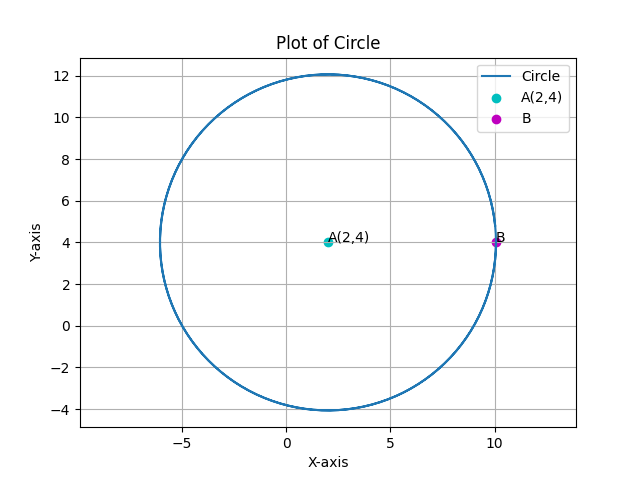
\includegraphics[width=0.7\linewidth]{figs/fig.png}
  \caption{Plot of the Circle}
   \label{stemplot}
\end{figure}
\end{document}

